
%%%%%%%%%%%%%%%%%%%%%%%%%%%%%%%%%%%%%%%%%%%%%%%%%%%%%%
%%%%%%%%%%%%%%%%%%%%%%%%%%%%%%%%%%%%%%%%%%%%%%%%%%%%%%

\section{Properties and Flavors (P. Brisk, F. Rastello)}
\begin{frame}
\frametitle{Def-Use and Use-Def Chains}
\begin{itemize}
\item Def-Use chains: for a definition the set of all its uses
\item Use-Def chain: for a use the (unique under SSA) definition that reaches the use
\item direct connections to propagate data-flow information
\end{itemize}
\begin{minipage}[t]{0.5\textwidth}
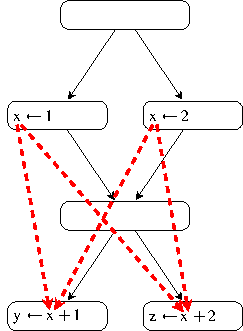
\includegraphics[valign=t,scale=0.65]{du-1}\hfill
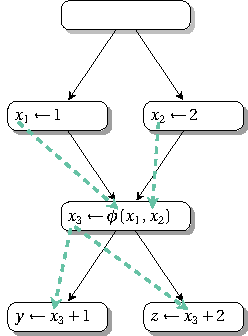
\includegraphics[valign=t,scale=0.65]{du-2}
\end{minipage}
\begin{minipage}[t]{0.48\textwidth}
\begin{itemize}
\item Information is combined as early as possible
\item Use-Def Chains for free; Def-Use Chains almost for free. 
\end{itemize}
\end{minipage}
\end{frame}

\begin{frame}
\frametitle{Minimality}
\begin{itemize}
\item Construction: place $\phi$-functions (e.g. $a=\phi(a,a)$); rename variables. Minimality is a property of the code \emph{before renaming}.
\item \emph{Single reaching-definition property}: no program point can be reached
by two definitions of the same variable
\item \emph{Minimality property}: minimality of the number of inserted $\phi$-functions
\item $n_3$ is a \emph{join node}  of $n_1$ and $n_2$ ($n_3\in {\cal J}(n_1,n_2)$) if $\exists$ two non-empty path (at least one edge), from $n_1$ to $n_3$ and from $n_2$ to $n_3$. 
\item \emph{necessary}: place $\phi$-functions of var $v$ at ${\cal J}(\textrm{Defs}_v)$
\item \emph{sufficient}: ${\cal J}(S \cup{\cal J}(S))={\cal J}(S)$
\item \emph{strictness}: in practice place at   ${\cal J}(\textrm{Defs}_v\cup r)$ 
\end{itemize}
\begin{minipage}{0.7\textwidth}
\begin{alertblock}{}
Minimality \emph{not} a requirement. Copy-propagation is enough.
\end{alertblock}
\end{minipage}
\end{frame}

\begin{frame}
\frametitle{Strict SSA Form and Dominance Property}
\begin{itemize}
\item \emph{strict}: if every variable is defined before it is used. Java imposes strictness, C++ does not.
\item $n_1$ \emph{dominates} basic block $n_2$ if every path
from $r$ to $n_2$ includes $n_1$
\end{itemize}
\begin{minipage}[t]{0.5\textwidth}
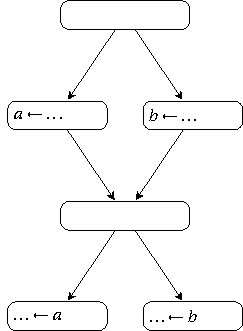
\includegraphics[valign=t,scale=0.65]{double-diamond-1}\hfill
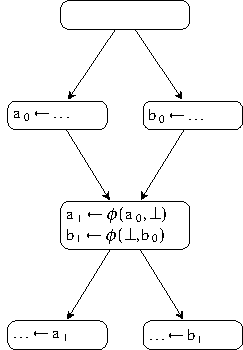
\includegraphics[valign=t,scale=0.65]{double-diamond-2}
\end{minipage}
\begin{minipage}[t]{0.45\textwidth}
\begin{itemize}
\item \emph{dominance property}: each use of a variable is dominated
by its definition
\item Add (undefined) pseudo-definition of each variable at $r$
\end{itemize}
\hspace{1cm}\goto{DomTree}{Dominator Tree}{2.5cm}
\end{minipage}
\end{frame}

\begin{frame}
\frametitle{Strict SSA Form and Dominance Property}
\begin{itemize}
\item So called ``\emph{Minimal SSA}'' (minimality and dominance property) can be efficiently built using formalism of \emph{dominance frontier} (${\cal J}(\textrm{Def}_v,r)=\textrm{DF}^+(v)$)
\item Structural properties of variables' live-range: sub-tree of the dominator tree ~~\goto{chordal}{Chordal}{1.4cm}
\begin{enumerate}
\item Fast liveness-check and iteration free liveness-set
\item Graph Coloring in linear time using \emph{tree scan} (register allocation)
\goto{spilltest}{Tree scan}{1.6cm}\end{enumerate}
\item \emph{break strictness}: e.g. copy-propagation
\item \emph{make it strict}: use standard incremental update
\end{itemize}
\begin{minipage}{0.5\textwidth}
\begin{alertblock}{}
Strictness is good especially for JIT
\end{alertblock}
\end{minipage}
\end{frame}

\begin{frame}
\frametitle{Pruned SSA Form}
\begin{itemize}
\item \emph{Minimal SSA}: $\phi$-functions where var not live prior to SSA construction
\end{itemize}
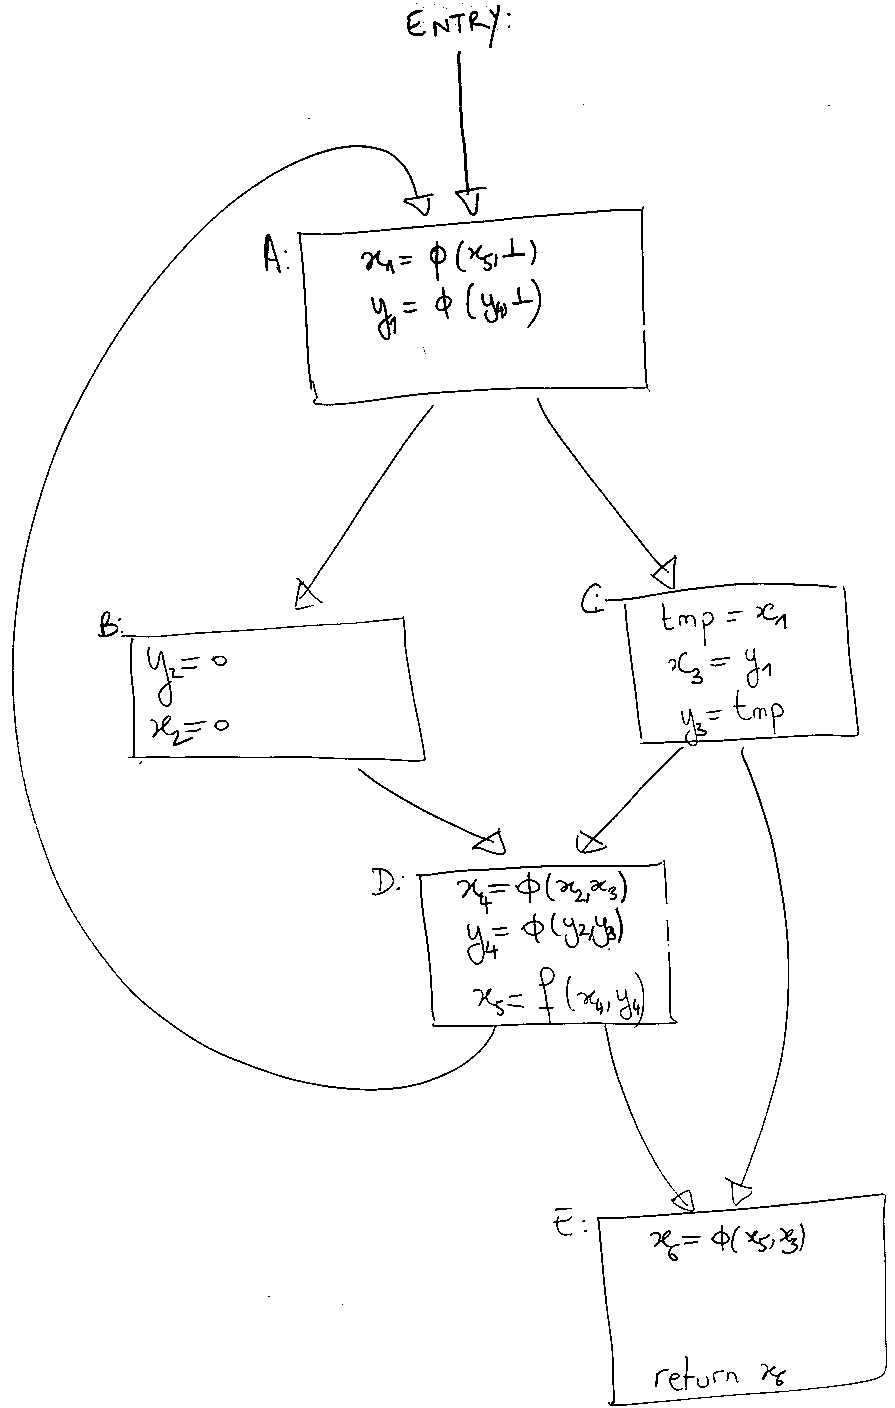
\includegraphics[valign=t,scale=0.63]{pruned}
\hspace{-0.8cm}\begin{minipage}[t]{0.47\textwidth}
\begin{itemize}
\item \emph{bad} for register allocation\\ \emph{good} for value numbering
\item \emph{pruned SSA}: without non-live $\phi$-functions
\item \emph{make it pruned}: dead-code elimination
\end{itemize}
\begin{alertblock}{}
Prune it (semi-pruned is ok) unless you \emph{really} need it
\end{alertblock}
\end{minipage}
\end{frame}

\begin{frame}
\frametitle{Conventional and Transformed SSA Form}
\begin{itemize}
\item \emph{register web}: maximum unions of def-use chains
\item \emph{$\phi$-webs}: transitive closure of $\phi$-related variables 
\end{itemize}
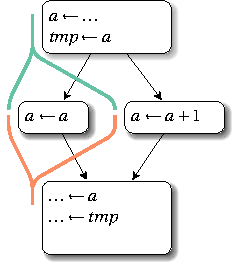
\includegraphics[valign=t,width=0.25\textwidth]{web-1}\hfill
\uncover<2->{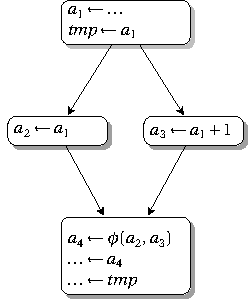
\includegraphics[valign=t,width=0.25\textwidth]{web-2}}\hfill
\uncover<3>{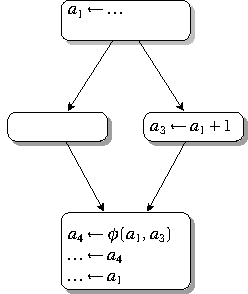
\includegraphics[valign=t,width=0.25\textwidth]{web-3}}
\begin{itemize}
\item<2-> \emph{Conventional SSA (C-SSA)}: each $\phi$-web is interference free. 
\item<3> \emph{Transformed SSA (T-SSA)}: non-conventional SSA
\end{itemize}
\end{frame}

\begin{frame}
\frametitle{Conventional and Transformed SSA Form}
\begin{itemize}
\item \emph{freshly constructed SSA}: $\phi$-web $\equiv$ register web of original non-SSA
\item \emph{destructing C-SSA}: replace each $\phi$-web by a single variable
\item \emph{make it conventional}: as ``difficult'' as destructing SSA: insert copies to dissociate interfering vars from the connecting $\phi$-functions.
\end{itemize}
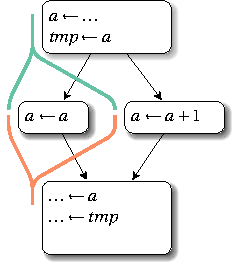
\includegraphics[valign=t,width=0.25\textwidth]{web-1}\hfill
\uncover{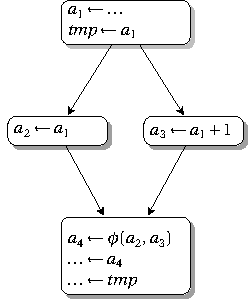
\includegraphics[valign=t,width=0.25\textwidth]{web-2}}\hfill
\uncover{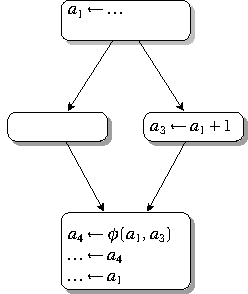
\includegraphics[valign=t,width=0.25\textwidth]{web-3}}
\begin{minipage}{0.7\textwidth}
\begin{alertblock}{}
\emph{Don't} try to enforce conventional property but for the really last phases of code generation
\end{alertblock}
\end{minipage}
\end{frame}


